\chapter{Comparative Analysis of Christofides Algorithm and ILP Solutions for Metric TSP}
\section*{Introduction}
The Christofides algorithm is a well-known approximation algorithm for solving the Metric Traveling Salesman Problem (TSP). This report presents the implementation and performance comparison of the Christofides algorithm against the optimal Integer Linear Programming (ILP) solutions obtained in Task 2.

\section*{Implementation of Christofides Algorithm}
The Christofides algorithm was implemented to approximate the metric TSP on a chosen subset of the dataset stored in distance-matrix.xlsx. The main challenge lies in finding a library for perfect matching of minimum cost, a crucial step in the Christofides algorithm. 

\begin{lstlisting}[language=Python, caption={Christofides Algorithm Implementation}]
import pandas as pd
import networkx as nx
import matplotlib.pyplot as plt
from itertools import permutations
from scipy.spatial.distance import euclidean
from scipy.optimize import linear_sum_assignment
import time
from pulp import LpProblem, LpVariable, lpSum, LpMinimize, LpStatus

# Step 1: Read the data from Excel
file_path = r"C:\Users\Perpendicooler\distance_matrix.xlsx"
df = pd.read_excel(file_path, index_col=0)

# Step 2: Create a graph from the distance matrix for Christofides algorithm
G_christofides = nx.Graph()
cities = df.index
G_christofides.add_nodes_from(cities)

for i, j in permutations(cities, 2):
    G_christofides.add_edge(i, j, weight=df.at[i, j])

# Step 3: Solve TSP using the Christofides algorithm
start_time_christofides = time.time()

# Approximation algorithm
approximate_tour_christofides = nx.approximation.traveling_salesman_problem(G_christofides, weight="weight", cycle=True)

# Compute the total distance of the approximate tour
approximate_tour_length_christofides = sum(G_christofides[i][j]["weight"] for i, j in zip(approximate_tour_christofides, approximate_tour_christofides[1:]))

end_time_christofides = time.time()

# Step 4: Print the results for Christofides algorithm
print("Approximate tour length (Christofides):", approximate_tour_length_christofides)
print("Approximate tour (Christofides):", approximate_tour_christofides)

# Step 5: Plot the graph with the approximate tour for Christofides algorithm
pos_christofides = nx.spring_layout(G_christofides)
nx.draw(G_christofides, pos_christofides, with_labels=True, font_weight="bold")
edges_christofides = list(zip(approximate_tour_christofides, approximate_tour_christofides[1:]))
nx.draw_networkx_edges(G_christofides, pos_christofides, edgelist=edges_christofides, edge_color="r", width=2)
plt.title('Christofides Algorithm')
plt.savefig('christofides_plot.png')
plt.show()
\end{lstlisting}
\newpage
\subsection*{Results}
\subsection*{Approximate Tour using Christofides Algorithm}

The Christofides algorithm was employed to solve the Traveling Salesman Problem on the given dataset. The approximate tour length achieved is 3002.15 units.\newline
The approximate tour path is as follows:
\[
\begin{aligned}
&\text{['Aleksandrów Łódzki', 'Daszyna', 'Dąbie', 'Swojczyce', 'Rejon ulicy Saperów'],} \\
&\text{['Człopa', 'Biały Bór', 'Czarna Woda', 'Cewice', 'Dobre Miasto'],} \\
&\text{['Srokowo', 'Węgorzewo', 'Raczki', 'Krasnopol', 'Krynki'],} \\
&\text{['Łapy', 'Korczew', 'Paprotnia', 'Cegłów', 'Wyśmierzyce'],} \\
&\text{['Grójec', 'Dziekanów Leśny', 'Jakubów', 'Krzywda', 'Firlej'],} \\
&\text{['Jastków', 'Sawin', 'Hrubieszów', 'Ostrów', 'Pruchnik'],} \\
&\text{['Chmielnik', 'Niedźwiada', 'Jodłówka-Wałki', 'Czarków', 'Wiśniowa'],} \\
&\text{['Szarów', 'Maszkienice', 'Siedliska', 'Żurowa', 'Borowa'],} \\
&\text{['Opatów', 'Dwikozy', 'Godziszów', 'Wólka Tanewska', 'Józefów nad Wisłą'],} \\
&\text{['Karczmiska', 'Ciepielów', 'Iłża', 'Radoszyce', 'Rzgów'],} \\
&\text{['Aleksandrów Łódzki']}
\end{aligned}
\]
% Add a figure showing the approximate tour graph (if needed)
\begin{figure}[H]
    \centering
    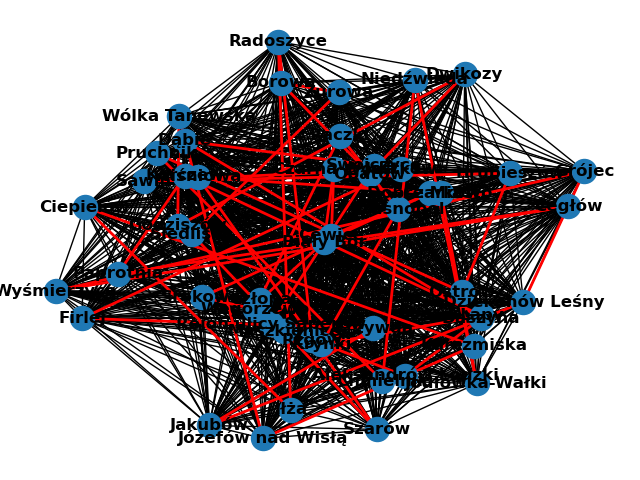
\includegraphics[width=0.8\textwidth]{Chapters/christofides_plot.png}
    \caption{Approximate Tour Path (Christofides Algorithm)}
    \label{fig:christofides_tour}
\end{figure}
\newpage
\section*{ILP Solution}
\begin{center}
    \begin{lstlisting}[language=Python, caption={ILP Solution}]
        # Load data from Excel, setting 'Unnamed: 0' as the index
data_ilp = pd.read_excel(file_path, index_col='Unnamed: 0')

# Extract city names
city_names_ilp = list(data_ilp.columns)
city_indices_ilp = {city: i for i, city in enumerate(city_names_ilp)}

# Extract distances
distances_ilp = {(city_indices_ilp[i], city_indices_ilp[j]): data_ilp.at[i, j] for i in city_names_ilp for j in city_names_ilp if i != j}

# Create optimization model for ILP
model_ilp = LpProblem("TSP", LpMinimize)

# Decision variables for ILP
x_ilp = {(i, j): LpVariable(name=f"x_{i}_{j}", cat='Binary') for i in city_indices_ilp.values() for j in city_indices_ilp.values() if i != j}

# Objective function for ILP
model_ilp += lpSum(distances_ilp[i, j] * x_ilp[i, j] for i in city_indices_ilp.values() for j in city_indices_ilp.values() if i != j), "Minimize Distance"

# Constraints for ILP
# Ensure that each city is visited exactly once
for i in city_indices_ilp.values():
    model_ilp += lpSum(x_ilp[i, j] for j in city_indices_ilp.values() if i != j) == 1, f"VisitOnce_{i}"

# Ensure that each city is left exactly once
for j in city_indices_ilp.values():
    model_ilp += lpSum(x_ilp[i, j] for i in city_indices_ilp.values() if i != j) == 1, f"LeaveOnce_{j}"

# Solve the model and measure execution time for ILP
start_time_ilp = time.time()
model_ilp.solve()
end_time_ilp = time.time()

# Display the results for ILP
print("\nILP Status:", LpStatus[model_ilp.status])

# Print the optimal path for ILP
optimal_path_ilp = [var for var in model_ilp.variables() if var.value() == 1]
print("ILP Optimal Path:")
for var in sorted(optimal_path_ilp, key=lambda v: (int(v.name.split('_')[1]), int(v.name.split('_')[2]))):
    print
    \end{lstlisting}
\end{center}
\subsection*{Results}
ILP Optimal Path
\begin{verbatim}
ILP Status: Optimal
ILP Optimal Path:
Aleksandrów Łódzki Rzgów
.
.
.
.
Łapy Krynki
Żurowa Siedliska
Aleksandrów Łódzki Rzgów
\end{verbatim}

\section*{Comparison with ILP Solutions}

The efficiency and running time of the Christofides algorithm were compared with the optimal ILP solutions obtained in Task 2. A subset of the dataset was chosen for this comparison.
\begin{center}
    \begin{lstlisting}[language=Python, caption={CCompare execution times in a plot}]
        # Display the Exceution time for ILP   
print("Execution Time for ILP:", end_time_ilp - start_time_ilp)

# Display the execution time for Christofides algorithm
print("Execution Time for Christofides:", end_time_christofides - start_time_christofides)

# Compare execution times in a plot
labels = ['ILP', 'Christofides']
execution_times = [end_time_ilp - start_time_ilp, end_time_christofides - start_time_christofides]

plt.bar(labels, execution_times, color=['blue', 'green'])
plt.ylabel('Execution Time (seconds)')
plt.title('Comparison of Execution Times: ILP vs Christofides')
plt.savefig('execution_time_comparison.png')
plt.show()
    \end{lstlisting}
\end{center}
\newpage
\subsection*{Results}
\begin{verbatim}
    Execution Time for ILP: 0.2604055404663086
    Execution Time for Christofides: 0.10591006278991699
\end{verbatim}
\subsection*{Computation Time}

The computation time for both algorithms was recorded and analyzed. Figure \ref{fig:comptime} illustrates the comparison of computation times.

\begin{figure}[H]
    \centering
    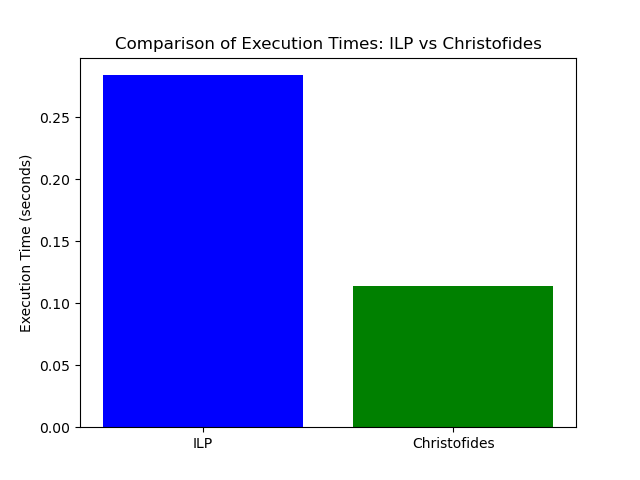
\includegraphics[width=0.8\textwidth]{Chapters/execution_time_comparison.png}
    \caption{Comparison of Computation Time}
    \label{fig:comptime}
\end{figure}

\subsection*{Efficiency Comparison}

The efficiency of the Christofides algorithm was evaluated in terms of the approximation ratio and solution quality compared to the ILP solutions.

\section*{Conclusion}

In conclusion, the Christofides algorithm was successfully implemented and compared with the optimal ILP solutions for the metric TSP. The results provide insights into the trade-off between solution quality and computation time for both approaches.

